


\documentclass[aspectratio=169,xcolor=dvipsnames]{beamer}
%\usetheme{SimplePlus}

\usepackage{hyperref}
\usepackage{graphicx} % Allows including images
\usepackage{booktabs} % Allows the use of \toprule, \midrule and \bottomrule in tables

%----------------------------------------------------------------------------------------
%	TITLE PAGE
%----------------------------------------------------------------------------------------

\title[Flowmåling] {strømningsmåling}
%\subtitle{Subtitle}

\author[Fred-Olav] {Fred-Olav Mosdal}

\institute[Gand VGS] % Your institution as it will appear on the bottom of every slide, may be shorthand to save space
{
    Gand VGS \\
    VG3 Automasjon
}
\date{\today} % Date, can be changed to a custom date
\begin{document}
\maketitle

%\subsection{Fluid viscosity}
\begin{frame}
	\frametitle{Fluid viskositet}

	


%
%\textit{Viscosity} is a measure of a fluid's resistance to shear.  It may be visualized as a sort of internal friction, where individual fluid molecules experience either cohesion or collision while flowing past one another.  The more ``viscous'' a fluid is, the ``thicker'' it is when stirred.  Clean water is an example of a low-viscosity liquid, while liquid honey at room temperature is an example of a high-viscosity liquid.  \index{Viscosity}
%
%There are two different ways to quantify the viscosity of a fluid: \textit{absolute viscosity} and \textit{kinematic viscosity}.  Absolute viscosity (symbolized by the Greek symbol ``eta'' $\eta$, or sometimes by the Greek symbol ``mu'' $\mu$), also known as \textit{dynamic viscosity}, is a direct relation between stress placed on a fluid and its rate of deformation (or shear).  The textbook definition of absolute viscosity is based on a model of two flat plates moving past each other with a film of fluid separating them.  The relationship between the shear stress applied to this fluid film (force divided by area) and the velocity/film thickness ratio is viscosity:  \index{Viscosity, absolute} \index{Viscosity, kinematic} \index{Absolute viscosity} \index{Kinematic viscosity}
%
	$$\includegraphics[width=9cm]{fluids_09.eps}$$
%
$$\eta = {FL \over Av}$$
%
%\noindent
%Where,
%
$\eta$ = Absolute viscosity (pascal-seconds), also symbolized as $\mu$ 
%
$F$ = Force (newtons)
%
$L$ = Film thickness (meters) -- typically \textit{much} less than 1 meter for any realistic demonstration!
%
$A$ = Plate area (square meters)
%
$v$ = Relative velocity (meters per second)
%
\end{frame}
%\vskip 10pt
%
%Another common unit of measurement for absolute viscosity is the \textit{poise}, with 1 poise being equal to 0.1 pascal-seconds.  Both units are too large for common use, and so absolute viscosity is often expressed in \textit{centipoise}.  Water has an absolute viscosity of very nearly 1.000 centipoise.  \index{Poise}
%
%\vskip 10pt
%
%\filbreak
\begin{frame}
	\frametitle{Kinematisk viskositet}

	


%
%Kinematic viscosity (symbolized by the Greek letter ``nu'' $\nu$) includes an assessment of the fluid's density in addition to all the above factors.  It is calculated as the quotient of absolute viscosity and mass density:
%
$$\nu = {\eta \over \rho}$$
%
%\noindent
%Where,
%
$\nu$ = Kinematic viscosity (stokes)
%
$\eta$ = Absolute viscosity (poise)
%
$\rho$ = Mass density (grams per cubic centimeter)
%
%\vskip 10pt
%
\end{frame}
%As with the unit of poise, the unit of stokes is too large for convenient use, so kinematic viscosities are often expressed in units of \textit{centistokes}.  Water has a kinematic viscosity of very nearly 1.000 centistokes.  \index{Stokes}
%
%\vskip 10pt
%
%The mechanism of viscosity in liquids is inter-molecular \textit{cohesion}.  Since this cohesive force is overcome with increasing temperature, most liquids tend to become ``thinner'' (less viscous) as they heat up.  The mechanism of viscosity in gases, however, is inter-molecular \textit{collisions}.  Since these collisions increase in frequency and intensity with increasing temperature, gases tend to become ``thicker'' (more viscous) as they heat up. \index{Viscosity, temperature dependence}
%
%As a ratio of stress to strain (applied force to yielding velocity), viscosity is often constant for a given fluid at a given temperature.  Interesting exceptions exist, though.  Fluids whose viscosities change with applied stress, and/or over time with all other factors constant, are referred to as \textit{non-Newtonian fluids}.  A simple example of a non-Newtonian fluid is cornstarch mixed with water, which ``solidifies'' under increasing stress and then returns to a liquid state when the stress is removed.  \index{Non-Newtonian fluid}
%
%
%
%
%
%
%
%\filbreak
\begin{frame}
	\frametitle{Reynolds nummer}

	


%\subsection{Reynolds number}
%
%\textit{Viscous flow} is a condition where friction forces dominate the behavior of a moving fluid, typically in cases where viscosity (internal fluid friction) is great.  \textit{Inviscid flow}, by contrast, is a condition where friction within a moving fluid is negligible and the fluid moves freely.  The \textit{Reynolds number} of a fluid is a dimensionless quantity expressing the ratio between a moving fluid's momentum and its viscosity, and is a helpful gauge in predicting how a fluid stream will move.  \index{Viscous flow} \index{Inviscid flow} \index{Reynolds number}
%
%\label{Reynolds number}
%
%A couple of formulae for calculating Reynolds number of a flow are shown here:
%
$$\hbox{Re} = {{D \overline{v} \rho} \over \mu}$$
%
%\noindent
%Where,
%
Re = Reynolds number (unitless)
%
$D$ = Diameter of pipe, (meters)
%
$\overline{v}$ = Average velocity of fluid (meters per second)
%
$\rho$ = Mass density of fluid (kilograms per cubic meter)
%
$\mu$ = Absolute viscosity of fluid (pascal-seconds)
%
\end{frame}
%\vskip 20pt
%
%$$\hbox{Re} = {{(3160) G_f Q} \over {D \mu}}$$
%
%\noindent
%Where,
%
%Re = Reynolds number (unitless)
%
%$G_f$ = Specific gravity of liquid (unitless)
%
%$Q$ = Flow rate (gallons per minute)
%
%$D$ = Diameter of pipe (inches)
%
%$\mu$ = Absolute viscosity of fluid (centipoise)
%
%3160 = Conversion factor for British units
%
%\vskip 10pt
%
%\filbreak
%
%The first formula, with all metric units, is the textbook ``definition'' for Reynolds number.  If you take the time to dimensionally analyze this formula, you will find that all units do indeed cancel to leave the Reynolds number unitless:
%
%$$\hbox{Re} = {{D \overline{v} \rho} \over \mu}$$
%
%$$\hbox{Re} = {{[\hbox{m}] \left[{\hbox{m} \over \hbox{s}}\right] \left[{\hbox{kg} \over \hbox{m}^3}\right] \over {[\hbox{Pa} \cdot \hbox{s}]}}}$$
%
%Recalling that the definition of a ``pascal'' is one Newton of force per square meter:
%
%$$\hbox{Re} = {\left[{\hbox{kg} \over {\hbox{m} \cdot \hbox{s}}}\right] \over \left[{\hbox{N} \cdot \hbox{s} \over \hbox{m}^2}\right]}$$
%
%$$\hbox{Re} = {\left[{\hbox{kg} \over {\hbox{m} \cdot \hbox{s}}}\right] \cdot \left[{\hbox{m}^2 \over \hbox{N} \cdot \hbox{s}}\right]}$$
%
%$$\hbox{Re} = \left[{{\hbox{kg} \cdot \hbox{m}} \over {\hbox{N} \cdot \hbox{s}^2}}\right]$$
%
%Recalling that the definition of a ``newton'' is one kilogram times meters per second squared (from Newton's Second Law equation $F = ma$):
%
%$$\hbox{Re} = \left[{{\hbox{kg} \cdot \hbox{m} \cdot \hbox{s}^2} \over {\hbox{kg} \cdot \hbox{m} \cdot \hbox{s}^2}}\right]$$
%
%$$\hbox{Re} = \hbox{\textit{unitless}}$$
%
%\filbreak
%
%The second formula given for calculating Reynolds number includes a conversion constant of 3160, which bears the unwieldy unit of ``inches-centipoise-minutes per gallon'' in order that the units of all variables (flow in gallons per minute, pipe diameter in inches, and viscosity in centipoise) may cancel.  Note that specific gravity ($G_f$) is unitless and therefore does not appear in this dimensional analysis:  \index{Dimensional analysis}
%
%$$\hbox{Re} = {{(3160) G_f Q} \over {D \mu}}$$
%
%$$\hbox{Re} = { {{\left[{\hbox{in} \cdot \hbox{cp} \cdot \hbox{min}} \over \hbox{gal} \right]} \left[{\hbox{gal} \over \hbox{min}}\right]} \over {[\hbox{in} \cdot \hbox{cp}]}}$$
%
%$$\hbox{Re} = \hbox{\textit{unitless}}$$
%
%You will often find this formula, and the conversion constant of 3160, shown without units at all.  Its sole purpose is to make the calculation of Reynolds number easy when working with British units customary in the United States.
%
%\vskip 10pt
%
%\filbreak
%
%The Reynolds number of a fluid stream may be used to qualitatively predict whether the flow regime will be \textit{laminar} or \textit{turbulent}.  Low Reynolds number values predict laminar (viscous) flow, where fluid molecules move in straight ``stream-line'' paths, and fluid velocity near the center of the pipe is substantially greater than near the pipe walls:
\begin{frame}
	\frametitle{Laminær strømning}

	


%
$$\includegraphics{fluids_04.eps}$$
%
\end{frame}
\begin{frame}
	\frametitle{Turbulent strømning}

	



%High Reynolds number values predict turbulent (inviscid) flow, where individual molecule motion is chaotic on a microscopic scale, and fluid velocities across the face of the flow profile are similar:
%
$$\includegraphics{fluids_05.eps}$$
%
%It should be emphasized that this turbulence is microscopic in nature, and occurs even when the fluid flows through a piping system free of obstructions, rough surfaces, and/or sudden directional changes.  At high Reynolds number values, turbulence simply \textit{happens}.
%
%Other forms of turbulence, such as \textit{eddies} and \textit{swirl} are possible at high Reynolds numbers, but are caused by disturbances in the flow stream such as pipe elbows, tees, control valves, thermowells, and other irregular surfaces.  The ``micro-turbulence'' naturally occurring at high Reynolds numbers will actually randomize such macroscopic (large-scale) motions if the fluid subsequently passes through a long enough length of straight pipe.  
%
%Turbulent flow is actually the desired condition for many industrial processes.  When different fluids must be mixed together, for example, laminar flow is a bad thing: only turbulent flow will guarantee thorough mixing.  The same is true for convective heat exchange: in order for two fluids to effectively exchange heat energy within a heat exchanger, the flow must be turbulent so that molecules from all portions of the flow stream will come into contact with the exchanger walls.  Many types of flowmeters require a condition called \textit{fully-developed turbulent flow}, where the flow profile is relatively flat and the only turbulence is that existing on a microscopic scale.  Large-scale disturbances in the flow profile such as eddies and swirl tend to negatively affect the measurement performance of many flowmeter designs.  This is why such flowmeters usually require long lengths of ``straight-run'' piping both upstream and downstream: to give micro-turbulence the opportunity to randomize any large-scale motions and homogenize the velocity profile.  \index{Fully developed turbulent flow}
%
\end{frame}
%\filbreak
%
%A generally accepted rule-of-thumb is that Reynolds number values less than 2000 will probably be laminar, while values in excess of 10000 will probably be turbulent.  There is no definite threshold value for all fluids and piping configurations, though.  To illustrate, I will share with you some examples of Reynolds number thresholds for laminar versus turbulent flows given by various technical sources:  \index{Turbulent flow}  \index{Laminar flow}  \index{Reynolds number, for laminar versus turbulent flow regimes}
%
%\vskip 10pt
%
%\noindent
%\underbar{Chapter 2.8: Laminar Flowmeters} of the \textit{Instrument Engineers' Handbook, Process Measurement and Analysis, Third Edition} (pg. 105 -- authors: R. Siev, J.B. Arant, B.G. Lipt\'ak) define Re $<$ 2000 as ``laminar'' flow, Re $>$ 10000 as ``fully developed turbulent'' flow, and any Reynolds number values between 2000 and 10000 as ``transitional'' flow.
%
%\vskip 10pt
%
%\noindent
%\underbar{Chapter 2: Fluid Properties -- Part II} of the \textit{ISA Industrial Measurement Series -- Flow} (pg. 11) define ``laminar'' flow as Re $<$ 2000, ``turbulent'' flow as Re $>$ 4000, and any Reynolds values in between 2000 and 4000 as ``transitional'' flow.
%
%\vskip 10pt
%
%\noindent
%The \underbar{Laminar Flow in a Pipe} section in the \textit{Standard Handbook of Engineering Calculations} (pg. 1-202) defines ``laminar'' flow as Re $<$ 2100, and ``turbulent'' flow as Re $>$ 3000.  In a later section of that \textit{same book} (\underbar{Piping and Fluid Flow} -- page 3-384), ``laminar'' flow is defined as Re $<$ 1200 and ``turbulent'' flow as Re $>$ 2500.
%
%\vskip 10pt
%
%\noindent
%Douglas Giancoli, in his physics textbook \textit{Physics} (third edition, pg. 11), defines ``laminar'' flow as Re $<$ 2000 and ``turbulent'' flow as Re $>$ 2000.
%
%\vskip 10pt
%
%\noindent
%Finally, a source on the Internet (\texttt{http://flow.netfirms.com/reynolds/theory.htm}) attempts to define the threshold separating laminar from turbulent flow to an unprecedented degree of precision: Re $<$ 2320 is supposedly the defining point of ``laminar'' flow, while Re $>$ 2320 is supposedly marks the onset of ``turbulent'' flow.
%
%\vskip 10pt
%
%Clearly, Reynolds number alone is insufficient for consistent prediction of laminar or turbulent flow, otherwise we would find far greater consistency in the reported Reynolds number values for each regime.  Pipe roughness, swirl, and other factors influence flow regime, making Reynolds number an approximate indicator only.  It should be noted that laminar flow may be sustained at Reynolds numbers significantly in excess of 10000 under very special circumstances.  For example, in certain coiled capillary tubes, laminar flow may be sustained all the way up to Re = 15000, due to a phenomenon known as the \textit{Dean effect}!  \index{Dean effect}
%
%
%
%
%
%
%
%
%
%\filbreak
%\subsection{Law of Continuity}
\begin{frame}
	\frametitle{Kontunitetsloven, massestrøm}

	


%
%Any fluid moving through a pipe obeys the Law of Continuity, which states that the product of average velocity ($\overline{v}$), pipe cross-sectional area ($A$), and fluid density ($\rho$) for a given flow stream must remain constant:
%
%\label{Law of Continuity}
%
$$\rho_1 A_1 \overline{v_1} = \rho_2 A_2 \overline{v_2} = \cdots \rho_n A_n \overline{v_n}$$
%
$$\includegraphics{fluids_01.eps}$$
%
%Fluid continuity is an expression of a more fundamental law of physics: the \textit{Conservation of Mass}.  If we assign appropriate units of measurement to the variables in the continuity equation, we see that the units cancel in such a way that only units of mass per unit time remain:  \index{Conservation of Mass} \index{Law of Continuity (fluids)}
%
$$\rho A \overline{v} = \left[\hbox{kg} \over \hbox{m}^3\right] \left[\hbox{m}^2 \over 1 \right] \left[\hbox{m} \over \hbox{s} \right] = \left[\hbox{kg} \over \hbox{s} \right]$$
%
%This means we may define the product $\rho A \overline{v}$ as an expression of \textit{mass flow rate}, or $W$:
%
$$W = \rho A \overline{v}$$
%
\end{frame}
%In order for the product $\rho A \overline{v}$ to differ between any two points in a pipe, mass would have to mysteriously appear and disappear.  So long as the flow is continuous (not pulsing), and the pipe does not leak, it is impossible to have different rates of mass flow at different points along the flow path without violating the Law of Mass Conservation.  The continuity principle for fluid through a pipe is analogous to the principle of current being the same everywhere in a series-connected electric circuit, and for equivalently the same reason\footnote{The conservation law necessitating equal current at all points in a series electric circuit is the \textit{Law of Charge Conservation}, which states that electric charges cannot be created or destroyed.}.  \index{Conservation of Electric Charge}
%
%\vskip 10pt
%
%\filbreak
%
%We refer to a flowing fluid as \textit{incompressible} if its density does not substantially change with modest changes in pressure\footnote{Although not grammatically correct, this is a common use of the word in discussions of fluid dynamics.  By definition, something that is ``incompressible'' \textit{cannot} be compressed, but that is not how we are using the term here.  We commonly use the term ``incompressible'' to refer to either a moving liquid (in which case the actual compressibility of the liquid is inconsequential) or a gas/vapor that \textit{does not happen to undergo substantial compression or expansion as it flows through a pipe}.  In other words, an ``incompressible'' flow is a moving fluid whose $\rho$ does not substantially change, whether by actual impossibility or by circumstance.}.  For this limiting case, $\rho$ is constant and the continuity equation simplifies to the following form:  \index{Limiting case}
\begin{frame}
	\frametitle{Volumstrøm}

	


%
$$A_1 \overline{v_1} = A_2 \overline{v_2}$$
%
%Examining this equation in light of dimensional analysis, we see that the product $A \overline{v}$ is also an expression of flow rate:  \index{Dimensional analysis}
%
$$A \overline{v} = \left[\hbox{m}^2 \over 1 \right] \left[\hbox{m} \over \hbox{s} \right] = \left[\hbox{m}^3 \over \hbox{s} \right]$$
%
%Cubic meters per second is an expression of \textit{volumetric flow rate}, often symbolized by the variable $Q$:
%
$$Q = A \overline{v}$$
%
\end{frame}
%The practical implication of this principle is that fluid velocity is inversely proportional to the cross-sectional area of a pipe.  That is, fluid slows down when the pipe's diameter expands, and vice-versa.  We readily see this principle manifest in the natural world: rivers run slowest where they are deep and wide, and run fastest where they are shallow and narrow.  
%
%More specifically, we may say that the average velocity of a fluid through a pipe varies inversely with the square of the diameter, since cross-sectional area is proportional to the square of the pipe diameter.  For example, if fluid flows at a velocity of 2 feet per second through a 12-inch pipe, and that pipe extends to a narrower section only 6 inches (half the diameter of the wide section), the velocity at the narrower section will be \textit{four times} as great (8 feet per second), since the area of that skinnier section is one-quarter the area of the wider section.
%
%\filbreak
%
%For example, consider a pipe with an inside diameter of 8 inches (2/3 of a foot), passing a liquid flow of 5 cubic feet per minute.  The average velocity ($v$) of this fluid may be calculated as follows:
\begin{frame}
	\frametitle{Eksempel}

	


%
$$Q = A \overline{v}$$
%
$$\overline{v} = {Q \over A}$$
%
%Solving for $A$ in units of square feet:
%
$$A = \pi r^2$$
%
$$A = \pi \left({1 \over 3} \hbox{ ft}\right)^2 = {\pi \over 9} \hbox{ ft}^2$$
%
%Now, solving for average velocity $\overline{v}$:
%
$$\overline{v} = {Q \over A} = {{5 \hbox{ ft}^3 \over \hbox{min}} \over {{\pi \over 9} \hbox{ ft}^2}}$$
%
$$\overline{v} = \left({5 \hbox{ ft}^3 \over \hbox{min}}\right) \left({9 \over {\pi \hbox{ ft}^2}}\right)$$
%
$$\overline{v} = {45 \hbox{ ft} \over \pi \hbox{ min}} = 14.32 {\hbox{ft} \over \hbox{min}}$$
%
\end{frame}
%Thus, the average fluid velocity inside an 8-inch pipe passing a volumetric flow rate of 5 cubic feet per minute is 14.32 feet per minute.

%\subsection{Viscous flow}
\begin{frame}
	\frametitle{Viskos strømning}

	


%
%The pressure dropped by a slow-moving, viscous fluid through a pipe is described by the \textit{Hagen-Poiseuille equation}.  This equation applies only for conditions of low Reynolds number; i.e. when viscous forces are the dominant restraint to fluid motion through the pipe, and turbulence is nonexistent:  \index{Hagen-Poiseuille equation} \index{Laminar flow}
%
$$Q = k \left({{\Delta P D^4} \over {\mu L}}\right)$$
%
%\noindent
%Where,
%
$Q$ = Flow rate (gallons per minute)
%
$k$ = Unit conversion factor = 7.86 $\times 10^5$
%
$\Delta P$ = Pressure drop (inches of water column)
%
$D$ = Pipe diameter (inches)
%
$\mu$ = Liquid viscosity (centipoise) -- this is a temperature-dependent variable!
%
$L$ = Length of pipe section (inches)
%
\end{frame}
%\vskip 10pt
%
%
%
%
%
%
%\filbreak
%\subsection{Bernoulli's equation}
\begin{frame}
	\frametitle{Bernoullis formel}

	


%
%\label{Bernoulli's equation}
%
%\textit{Bernoulli's equation} is an expression of the \textit{Law of Energy Conservation} for an inviscid (frictionless) fluid stream, named after Daniel Bernoulli\footnote{According to Ven Te Chow in \textit{Open Channel Hydraulics}, who quotes from Hunter Rouse and Simon Ince's work \textit{History of Hydraulics}, Bernoulli's equation was first formulated by the great mathematician Leonhard Euler and made popular by Julius Weisbach, not by Daniel Bernoulli himself.}.  It states that the sum total energy at any point in a passive fluid stream (i.e. no pumps or other energy-imparting machines in the flow path, nor any energy-dissipating elements) must be constant.  Two versions of the equation are shown here:  \index{Bernoulli's equation}  \index{Conservation of Energy}  \index{Bernoulli, Daniel}  \index{Euler, Leonhard}
%
$$z_1 \rho g + {v_1^2 \rho \over 2} + P_1 = z_2 \rho g + {v_2^2 \rho \over 2} + P_2$$
%
$$z_1 + {v_1^2 \over {2 g}} + {P_1 \over \gamma} = z_2 + {v_2^2 \over {2 g}} + {P_2 \over \gamma}$$
%
%\noindent
%Where,
%
$z$ = Height of fluid (from a common reference point, usually ground level)
%
$\rho$ = Mass density of fluid
%
$\gamma$ = Weight density of fluid ($\gamma = \rho g$)
%
$g$ = Acceleration of gravity
%
$v$ = Velocity of fluid
%
$P$ = Pressure of fluid
%
\end{frame}
%\vskip 10pt
%
%Each of the three terms in Bernoulli's equation is an expression of a different kind of energy, commonly referred to as \textit{head}: \index{Head (fluid)}
%
%$$z \rho g \hbox{\hskip 20pt Elevation head}$$
%
%$${v^2 \rho \over 2} \hbox{\hskip 20pt Velocity head}$$
%
%$$P \hbox{\hskip 20pt Pressure head}$$
%
%Elevation and Pressure heads are potential forms of energy, while Velocity head is a kinetic form of energy.  Note how the elevation and velocity head terms so closely resemble the formulae for potential and kinetic energy of solid objects:
%
%$$E_p = mgh \hbox{\hskip 20pt Potential energy formula}$$
%
%$$E_k = {1 \over 2}mv^2 \hbox{\hskip 20pt Kinetic energy formula}$$
%
%The only real differences between the solid-object and fluid formulae for energies is the use of mass \textit{density} ($\rho$) for fluids instead of mass ($m$) for solids, and the arbitrary use of the variable $z$ for height instead of $h$.  In essence, the elevation and velocity head terms within Bernoulli's equation come from the assumption of individual fluid molecules behaving as miniscule solid masses.
%
%\vskip 10pt
%
%It is very important to maintain consistent units of measurement when using Bernoulli's equation!  Each of the three energy terms (elevation, velocity, and pressure) \textit{must} possess the exact same units if they are to add appropriately\footnote{Surely you've heard the expression, ``Apples and Oranges don't add up.''  Well, pounds per square inch and pounds per square foot don't add up either!  A general mathematical rule in physics is that any quantities added to or subtracted from each other \textit{must} bear the exact same units.  This rule does not hold for multiplication or division, which is why we see units canceling in those operations.  With addition and subtraction, no unit cancellation occurs.}.  Here is an example of dimensional analysis applied to the first version of Bernoulli's equation (using British units):  \index{Dimensional analysis}
%
%$$z \rho g + {v^2 \rho \over 2} + P$$
%
%$$[\hbox{ft}] \left[\hbox{slug} \over \hbox{ft}^3\right] \left[\hbox{ft} \over \hbox{s}^2 \right] +  \left[\hbox{ft} \over \hbox{s} \right]^2 \left[\hbox{slug} \over \hbox{ft}^3\right] + \left[\hbox{lb} \over  \hbox{ft}^2\right] = \left[\hbox{slug} \over \hbox{ft} \cdot \hbox{s}^2 \right]$$
%
%As you can see, both the first and second terms of the equation (elevation and velocity heads) bear the same unit of slugs per foot-second squared after all the ``feet'' are canceled.  The third term (pressure head) does not appear as though its units agree with the other two terms, until you realize that the unit definition of a ``pound'' is a slug of mass multiplied by the acceleration of gravity in feet per second squared, following Newton's Second Law of motion ($F = ma$):
%
%$$[\hbox{lb}] = [\hbox{slug}] \left[\hbox{ft} \over \hbox{s}^2\right]$$
%
%Once we make this substitution into the pressure head term, the units are revealed to be the same as the other two terms, slugs per foot-second squared:
%
%$$\left[\hbox{lb} \over  \hbox{ft}^2\right] = \left[\hbox{slug} \left[\hbox{ft} \over \hbox{s}^2\right] \over  \hbox{ft}^2\right] = \left[\hbox{slug} \over \hbox{ft} \cdot \hbox{s}^2 \right]$$
%
%In order for our British units to be consistent here, we must use \textit{feet} for elevation, \textit{slugs} per cubic \textit{foot} for mass density, \textit{feet} per \textit{second} squared for acceleration, \textit{feet} per \textit{second} for velocity, and \textit{pounds} per square \textit{foot} for pressure.  If one wished to use the more common pressure unit of PSI (pounds per square inch) with Bernoulli's equation instead of PSF (pounds per square foot), all the other units would have to change accordingly: elevation in \textit{inches}, mass density in slugs per cubic \textit{inch}, acceleration in \textit{inches} per second squared, and velocity in \textit{inches} per second. 
%
%Just for fun, we can try dimensional analysis on the second version of Bernoulli's equation, this time using metric units:
%
%$$z + {v^2 \over {2 g}} + {P \over \gamma}$$
%
%$$[\hbox{m}] + \left[\left[\hbox{m} \over \hbox{s}\right]^2 \over \left[\hbox{m} \over \hbox{s}^2\right]\right] + \left[\left[\hbox{N} \over \hbox{m}^2 \right] \over \left[\hbox{N} \over \hbox{m}^3\right] \right] = [\hbox{m}]$$
%
%Here, we see that all three terms end up being cast in simple units of meters.  That is, the fluid's elevation, velocity, and pressure heads are all expressed as simple elevations.  In order for our metric units to be consistent here, we must use \textit{meters} for elevation, \textit{meters} per \textit{second} for velocity, \textit{meters} per \textit{second} squared for acceleration, \textit{pascals} (\textit{newtons} per square \textit{meter}) for pressure, and \textit{newtons} per cubic \textit{meter} for weight density.
%
%\vskip 10pt
%
%Applying Bernoulli's equation to real-life applications can be a bit daunting, as there are so many different units of measurement to contend with, and so many calculations which must be precise in order to arrive at a correct final answer.  The following example serves to illustrate how Bernoulli's equation may be applied to the solution of pressure at a point in a water piping system, assuming no frictional losses anywhere in the system:
%
%$$\includegraphics{fluids_12.eps}$$
\begin{frame}
	\frametitle{Oppgave}

	$$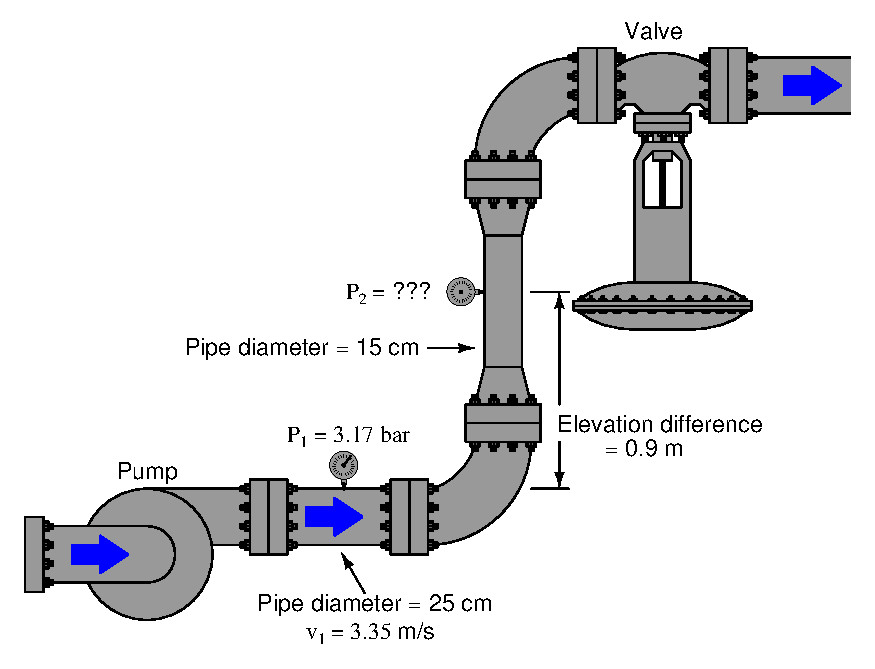
\includegraphics[height=7cm]{fluids_12x01.eps}$$
\end{frame}

%
%We know without a doubt that Bernoulli's equation will be what we need to evaluate in order to solve for the unknown pressure $P_2$, but where do we begin?  A good place to start is by writing the equation we know we will need, then identifying all known values and all unknown values:
%
%$$z_1 \rho g + {v_1^2 \rho \over 2} + P_1 = z_2 \rho g + {v_2^2 \rho \over 2} + P_2$$
%
%\filbreak
%
%Here is a list of known values, given to us already:
%
%% No blank lines allowed between lines of an \halign structure!
%% I use comments (%) instead, so that TeX doesn't choke.
%
%$$\vbox{\offinterlineskip
%\halign{\strut
%\vrule \quad\hfil # \ \hfil & 
%\vrule \quad\hfil # \ \hfil \vrule \cr
%\noalign{\hrule}
%%
%% First row
%\textbf{Known quantity} & \textbf{Comments} \cr
%%
%\noalign{\hrule}
%%
%% Another row
%$z_1$ & 0 ft (arbitrarily assigned as 0 height) \cr
%%
%\noalign{\hrule}
%%
%% Another row
%$z_2$ & 3 ft (if $z_1$ is 0 feet, then $z_2$ is 3 ft above it) \cr
%%
%\noalign{\hrule}
%%
%% Another row
%$v_1$ & 11 ft/s \cr
%%
%\noalign{\hrule}
%%
%% Another row
%$P_1$ & 46 PSI (\textit{need to convert into PSF so all units match}) \cr
%%
%\noalign{\hrule}
%%
%% Another row
%$g$ & 32.2. ft/s$^{2}$ \cr
%%
%\noalign{\hrule}
%} % End of \halign 
%}$$ % End of \vbox
%
%The conversion for $P_1$ from units of PSI into units of PSF is quite simple: multiply 46 PSI by 144 to get 6624 PSF.
%
%\vskip 10pt
%
%Here is a list of values unknown to us at this time:
%
%% No blank lines allowed between lines of an \halign structure!
%% I use comments (%) instead, so that TeX doesn't choke.
%
%$$\vbox{\offinterlineskip
%\halign{\strut
%\vrule \quad\hfil # \ \hfil & 
%\vrule \quad\hfil # \ \hfil \vrule \cr
%\noalign{\hrule}
%%
%% First row
%\textbf{Unknown quantity} & \textbf{Comments} \cr
%%
%\noalign{\hrule}
%%
%% Another row
%$\rho$ & (needs to be in units of slugs/ft$^{3}$) \cr
%%
%\noalign{\hrule}
%%
%% Another row
%$v_2$ & (needs to be in units of ft/s just like $v_1$) \cr
%%
%\noalign{\hrule}
%%
%% Another row
%$P_2$ & (the quantity we are ultimately solving for) \cr
%%
%\noalign{\hrule}
%} % End of \halign 
%}$$ % End of \vbox
%
%Now all we must do is solve for $\rho$ and $v_2$, and we will be ready to use Bernoulli's equation to solve for $P_2$.  The important of identifying all the known and unknown quantities \textit{before} beginning any calculations cannot be overstated.  Doing so allows us to \textit{develop a plan} for solving the problem.  Without a plan, one has no idea of where or how to proceed, which is a condition many students repeatedly find themselves in when solving physics-type problems.
%
%We know that $\rho$ is an expression of mass density for the fluid, and we were told the fluid in this example is water.  Water has a maximum density of 62.4 pounds per cubic foot, but this figure is not usable in our chosen form of Bernoulli's equation because it is \textit{weight} density ($\gamma$) and not \textit{mass} density ($\rho$).
%
%The relationship between weight density $\gamma$ and mass density $\rho$ is the exact same relationship between weight ($F_W$) and mass ($m$) in a gravitational field ($g$).  Newton's Second Law equation relating force to mass and acceleration ($F = ma$) works well to relate weight to mass and gravitational acceleration:
%
%$$F = ma$$
%
%$$F_W = mg$$
%
%Dividing both sides of this equation by volumetric units ($V$) (e.g. cubic feet) gives us our relationship between $\gamma$ and $\rho$:
%
%$${F_W \over V} = {m \over V} g$$
%
%$$\gamma = \rho g$$
%
%\filbreak
%
%Water has a weight density of 62.4 pounds per cubic foot in Earth gravity (32.2 feet per second squared), so:
%
%$$\rho = {\gamma \over g}$$
%
%$$\rho = {62.4 \hbox{ lb/ft}^3 \over 32.2 \hbox{ ft/s}^2} = 1.94 \hbox{ slugs/ft}^3$$
%
%Now we may calculate the total value for the left-hand side of Bernoulli's equation, representing the sum total of potential and kinetic heads for the fluid within the 10-inch pipe:
%
%$$z_1 \rho g + {v_1^2 \rho \over 2} + P_1 = \hbox{Total head at 10-inch pipe}$$
%
%% No blank lines allowed between lines of an \halign structure!
%% I use comments (%) instead, so Tex doesn't choke.
%
%$$\vbox{\offinterlineskip
%\halign{\strut
%\vrule \quad\hfil # \ \hfil & 
%\vrule \quad\hfil # \ \hfil & 
%\vrule \quad\hfil # \ \hfil \vrule \cr
%\noalign{\hrule}
%%
%% First row
%\textbf{Head} & \textbf{Calculation} at 10 inch pipe & \textbf{Value} \cr
%%
%\noalign{\hrule}
%%
%% Another row
%$z_1 \rho g$ & (0 ft) (1.94 slugs/ft$^{3}$) (32.2 ft/s$^{2}$) & 0 lb/ft$^{2}$ \cr
%%
%\noalign{\hrule}
%%
%% Another row
%$v_1^2 \rho / 2$ & (11 ft/s)$^{2}$ (1.94 slugs/ft$^{3}$) / 2 & 117.4 lb/ft$^{2}$ \cr
%%
%\noalign{\hrule}
%%
%% Another row
%$P_1$ & (46 lb/in$^{2}$) (144 in$^{2}$/1 ft$^{2}$) & 6624 lb/ft$^{2}$ \cr
%%
%\noalign{\hrule}
%%
%% Another row
%\textbf{Total} &  0 lb/ft$^{2}$ + 117.4 lb/ft$^{2}$ + 6624 lb/ft$^{2}$ & \textbf{6741.4 lb/ft$^{2}$} \cr
%%
%\noalign{\hrule}
%} % End of \halign 
%}$$ % End of \vbox
%
%Note the absolutely consistent use of units: all units of distance are \textit{feet}.  All units of mass as \textit{slugs}.  All units of time are \textit{seconds}.  Failure to maintain consistency of units will result in (often severely) incorrect results!\footnote{It is entirely possible to perform all our calculations using inches and/or minutes as the primary units instead of feet and seconds.  The only caveat is that \textit{all} units throughout all terms of Bernoulli's equation must be consistent.  This means we would also have to express mass density in units of slugs per cubic \textit{inch}, the acceleration of gravity in \textit{inches} per second squared (or \textit{inches} per \textit{minute} squared), and velocity in units of \textit{inches} per second (or \textit{inches} per \textit{minute}).  The only real benefit of doing this is that pressure would remain in the more customary units of pounds per square \textit{inch}.  My personal preference is to do all calculations using units of feet and seconds, then convert pressures in units of PSF to units of PSI at the very end.}
%
%\vskip 10pt
%
%\filbreak
%
%There is one more unknown quantity to solve for before we may calculate values at the 6-inch pipe, and that unknown quantity is $v_2$.  We know that the Continuity equation gives us a mathematical relationship between volumetric flow ($Q$), pipe area ($A$), and velocity ($v$):
%
%$$Q = A_1 v_1 = A_2 v_2$$
%
%Looking at this equation, the only variable we know the value of at this point is $v_1$, and we need to find $v_2$.  However, if we could find the values of $A_1$ and $A_2$, and/or $Q$, we would have the information we need to solve for $v_2$, which in turn would give us the information we would need to solve for $P_2$ in Bernoulli's equation.
%
%One way to approach this problem is to express the areas and velocities as ratios, eliminating $Q$ entirely so all we need to find are $A_1$ and $A_2$:
%
%$${A_1 \over A_2} = {v_2 \over v_1}$$
%
%The area of a circular pipe is given by the basic equation $A = \pi r^2$.  Since the problem gives us each pipe's diameter (10 inches and 6 inches), we know the radii (5 inches and 3 inches, respectively) which we may then plug into our ratio equation:
%
%$${\pi (5\hbox{ in})^2 \over \pi (3\hbox{ in})^2} = {v_2 \over v_1}$$
%
%$${25 \over 9} = {v_2 \over v_1}$$
%
%Knowing $v_1$ has a value of 11 feet per second, the solution for $v_2$ is now quite simple:
%
%$$v_2 = 11 \hbox{ ft/s} \left({25 \over 9}\right)$$
%
%$$v_2 = (11 \hbox{ ft/s}) (2.778) = 30.56 \hbox{ ft/s}$$
%
%\vskip 10pt
%
%\filbreak
%
%Finally, we have all the pieces necessary to solve for $P_2$ in the right-hand side of Bernoulli's equation:
%
%$$z_2 \rho g + {v_2^2 \rho \over 2} + P_2 = \hbox{Total head at 6-inch pipe}$$
%
%% No blank lines allowed between lines of an \halign structure!
%% I use comments (%) instead, so Tex doesn't choke.
%
%$$\vbox{\offinterlineskip
%\halign{\strut
%\vrule \quad\hfil # \ \hfil & 
%\vrule \quad\hfil # \ \hfil & 
%\vrule \quad\hfil # \ \hfil \vrule \cr
%\noalign{\hrule}
%%
%% First row
%\textbf{Head} & \textbf{Calculation} at 6 inch pipe & \textbf{Value} \cr
%%
%\noalign{\hrule}
%%
%% Another row
%$z_2 \rho g$ & (3 ft) (1.94 slugs/ft$^{3}$) (32.2 ft/s$^{2}$) & 187.4 lb/ft$^{2}$ \cr
%%
%\noalign{\hrule}
%%
%% Another row
%$v_2^2 \rho / 2$ & (30.56 ft/s)$^{2}$ (1.94 slugs/ft$^{3}$) / 2 & 905.6 lb/ft$^{2}$ \cr
%%
%\noalign{\hrule}
%%
%% Another row
%$P_2$ &  & (unknown) \cr
%%
%\noalign{\hrule}
%%
%% Another row
%\textbf{Total} & 187.4 lb/ft$^{2}$ + 905.6 lb/ft$^{2}$ + $P_2$ & \textbf{1093 lb/ft$^{2}$} + $P_2$ \cr
%%
%\noalign{\hrule}
%} % End of \halign 
%}$$ % End of \vbox
%
%Knowing that the total head calculated at the first location was 6741.4 lb/ft$^{2}$, and the Conservation of Energy requires total heads at both locations be equal (assuming no energy lost to fluid friction along the way), $P_2$ must be equal to:
%
%$$6741.4 \hbox{ lb/ft}^2 = 1093 \hbox{ lb/ft}^2 + P_2$$
%
%$$P_2 = 6741.4 \hbox{ lb/ft}^2 - 1093 \hbox{ lb/ft}^2 = 5648.3 \hbox{ lb/ft}^2$$
%
%Converting pounds per square foot into the more customary unit of pounds per square inch (PSI):
%
%$$P_2 = (5648.3 \hbox{ lb/ft}^2) \left({1 \hbox{ ft}^2 \over 144 \hbox{ in}^2}\right)$$
%
%$$P_2 = 39.2 \hbox{ lb/in}^2$$
%
%\filbreak
%
%Before discussing the larger meaning of our solution, it would be good to review the problem-solving plan we followed to calculate $P_2$:
%
%$$\includegraphics{fluids_34.eps}$$
%
%First, we identified Bernoulli's equation as being the central equation necessary for solving $P_2$.  Then, we identified all the known variables within Bernoulli's equation given to us in the problem, and also if there were any unit-conversion operations necessary.  Next, we identified any unknown variables necessary to solve for $P_2$ in Bernoulli's equation.  For each of those unknown variables, we found or developed equations to solve for them, based on variables known to us.  The graphic shown above illustrates our plan of solution, with arrows showing the dependent relationships where equations supplied values for unknown quantities in other equations.
%
%This is not just a problem-solving technique unique to Bernoulli's equation; it is a general strategy applicable to \textit{any} type of problem where multiple equations must be used to solve for some quantity.  The study of physics is general is filled with problems like this!
%
%\vskip 10pt
%
%\filbreak
%
%Note how our calculated value for $P_2$ at the second gauge is so much lower than the pressure at the first gauge: 39.2 PSI compared to 46 PSI.  This represents nearly a 7 PSI decrease in pressure!  Note also how little vertical distance separates the two gauges: only 3 feet.  Clearly, the change in elevation between those two points in insufficient to account for the large loss in pressure\footnote{A simple approximation for pressure loss due to elevation gain is approximately 1 PSI for every 2 vertical feet of water (1 PSI for every 27.68 inches to be more exact).}.  Given a 3 foot difference in elevation, one would expect a pressure reduction of about 1.3 PSI for a static column of water, but what we're seeing in this piping system is a pressure drop of nearly 7 PSI.  The difference is due to an exchange of energy from potential to kinetic form, as the fluid enters a much narrower pipe (6 inches instead of 10) and must increase velocity.
%
%Furthermore, if we were to increase the flow rate discharged from the pump, resulting in even more velocity through the narrow pipe, pressure at $P_2$ might even drop lower than atmospheric.  In other words, Bernoulli's equation tells us we can actually produce a \textit{vacuum} by accelerating a fluid through a constriction.  This principle is widely used in industry with devices known as \textit{eductors} or \textit{ejectors}\footnote{Technically, an \textit{eductor} uses a liquid such as water to generate the vacuum, while an \textit{ejector} uses a gas or a vapor such as steam.}: tapered tubes through which fluid flows at high velocity to produce a vacuum at the throat.    \index{Eductor}  \index{Ejector}  \index{Vacuum, produced by a venturi}
%
%$$\includegraphics{fluids_35.eps}$$
%
%This, in fact, is how a \textit{carburetor} works in an older automobile engine to vaporize liquid gasoline fuel into a stream of air drawn into the engine: the engine's intake air passes through a venturi tube, where vacuum at the throat of the venturi produces enough negative pressure to draw liquid gasoline into the stream to produce a fine mist.
%
%\filbreak
%
%Ejectors use a high-velocity gas or vapor (e.g. superheated steam) to produce significant vacuums.  Eductors use process liquid flow, such as the eductor shown in this next photograph where wastewater flow creates a vacuum to draw gaseous chlorine into the stream for biological disinfection:
%
%$$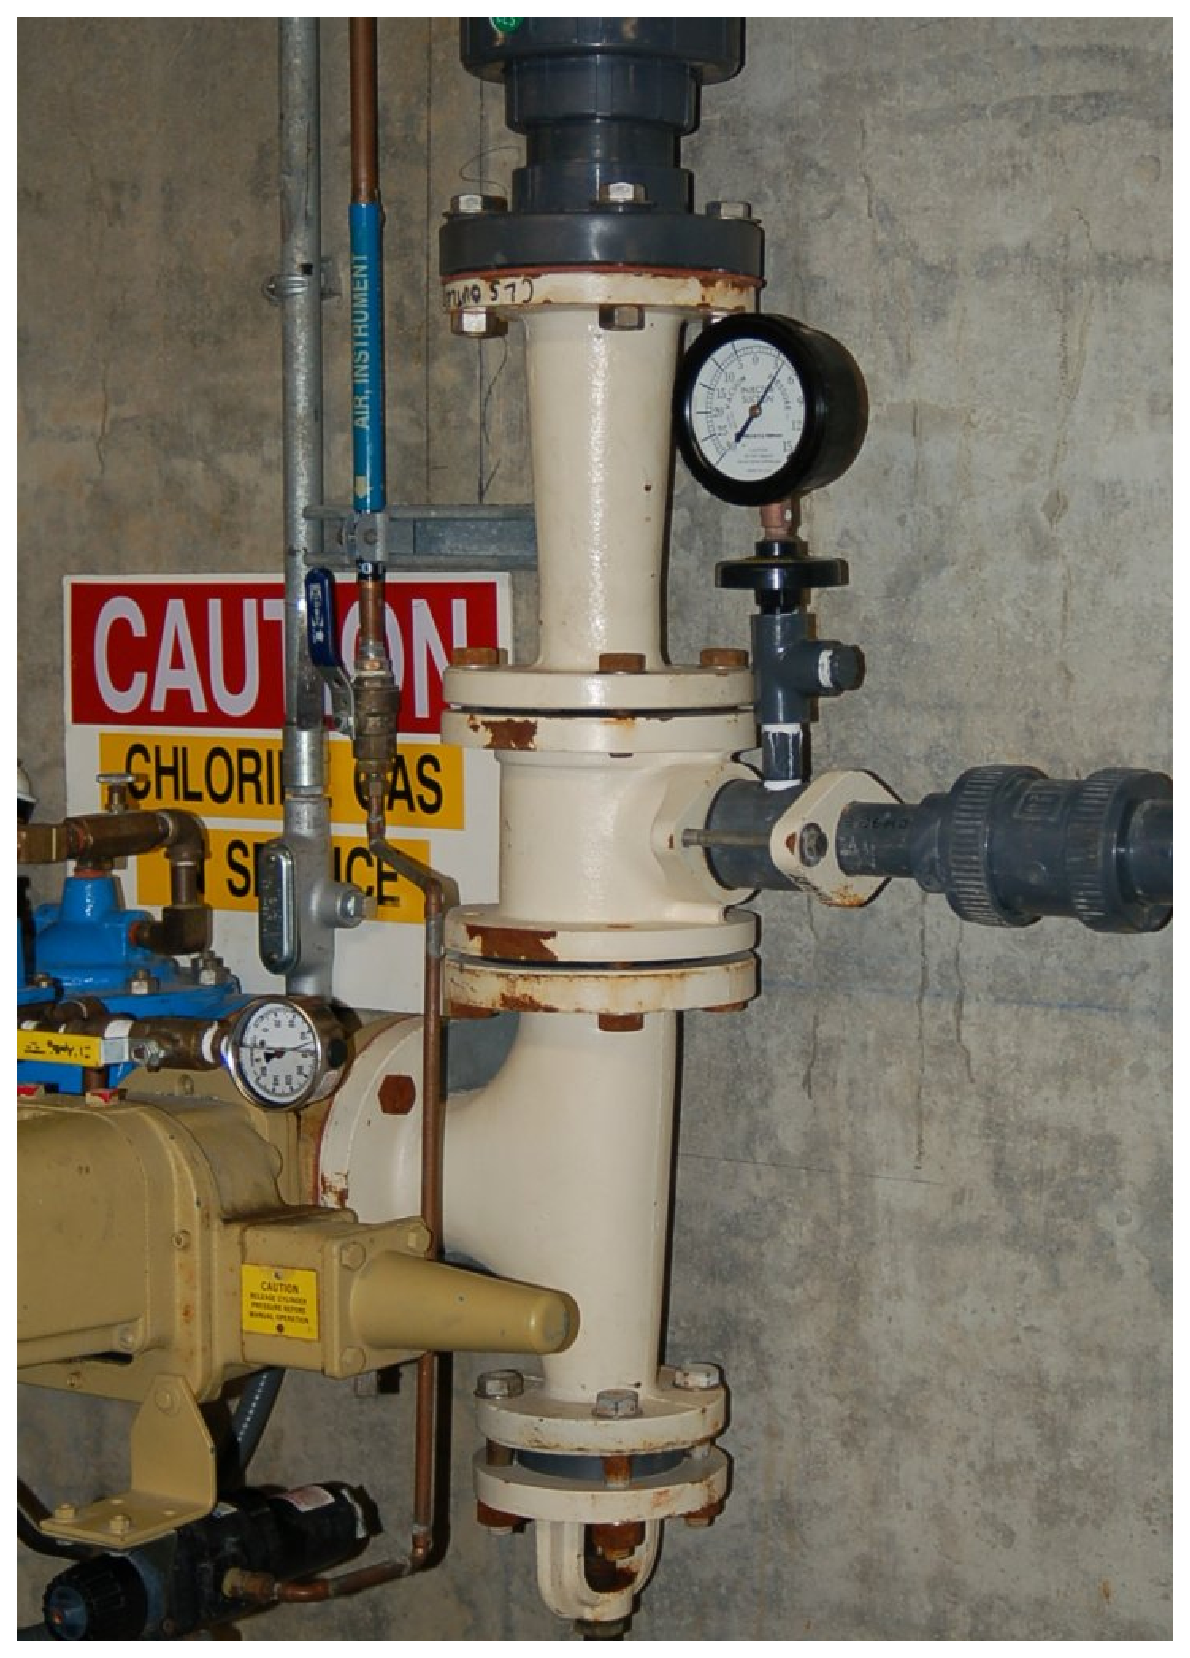
\includegraphics[height=5in]{fluids_20.eps}$$
%
%Here, the eductor helps fulfill an important safety function.  By creating a vacuum to draw toxic chlorine gas from the supply tank into the water stream, the chlorine gas piping may be continuously maintained at a slightly negative pressure throughout.  If ever a leak were to develop in the chlorine system, this vacuum would cause ambient air to enter the chlorine pipe rather than toxic chlorine gas to exit the pipe, making a leak far less dangerous than if the chlorine gas piping were maintained in a pressurized state.
%
%
%
%
%
%
%
%
%\filbreak
%\subsection{Torricelli's equation}
%
%The velocity of a liquid stream exiting from a nozzle, pressured solely by a vertical column of that same liquid, is equal to the free-fall velocity of a solid mass dropped from the same height as the top of the liquid column.  In both cases, potential energy (in the form of vertical height) converts to kinetic energy (motion):
%
%$$\includegraphics{fluids_02.eps}$$
%
%This was discovered by Evangelista Torricelli almost 100 years prior to Bernoulli's more comprehensive formulation.  The velocity may be determined by solving for $v$ after setting the potential and kinetic energy formulae equal to each other (since all potential energy at the upper height must translate into kinetic energy at the bottom, assuming no frictional losses): \index{Torricelli, Evangelista}
%
%$$mgh = {1 \over 2}mv^2$$
%
%$$gh = {1 \over 2}v^2$$
%
%$$2gh = v^2$$
%
%$$v = \sqrt{2gh}$$
%
%Note how mass ($m$) simply disappears from the equation, neatly canceling on both sides.  This means the nozzle velocity depends only on height, not the mass density of the liquid.  It also means the velocity of the falling object depends only on height, not the mass of the object.
%
%
%
%
%
%
%\filbreak
%\subsection{Flow through a venturi tube}
%
%If an incompressible fluid moves through a \textit{venturi tube} (i.e. a tube purposefully built to be narrow in the middle), the continuity principle tells us the fluid velocity must increase through the narrow portion.  This increase in velocity causes kinetic energy to increase at that point.  If the tube is level, there will be negligible difference in elevation ($z$) between different points of the tube's centerline, which means elevation head remains constant.  According to the Law of Energy Conservation, some other form of energy must decrease to account for the increase in kinetic energy.  This other form is the pressure head, which decreases at the throat of the venturi: \index{Venturi tube}
%
%$$\includegraphics{fluids_03.eps}$$
%
%Ideally, the pressure downstream of the narrow throat should be the same as the pressure upstream, assuming equal pipe diameters upstream and down.  However, in practice the downstream pressure gauge will show slightly less pressure than the upstream gauge due to some inevitable energy loss as the fluid passed through the venturi.  Some of this loss is due to fluid friction against the walls of the tube, and some is due to viscous losses within the fluid driven by turbulent fluid motion at the high-velocity throat passage.
%
%The difference between upstream and downstream pressure is called \textit{permanent pressure loss}, while the difference in pressure between the narrow throat and downstream is called \textit{pressure recovery}.  \index{Permanent pressure loss} \index{Pressure recovery}
%
%\filbreak
%
%If we install vertical sight-tubes called \textit{piezometers}\footnote{A piezometer tube is nothing more than a manometer (minus the well or the other half of the U-tube).} along a horizontal venturi tube, the differences in pressure will be shown by the heights of liquid columns within the tubes.  Here, we assume an ideal (inviscid) liquid with no permanent pressure loss:
%
%$$\includegraphics{fluids_06.eps}$$
%
%The height of liquid in each piezometer tube represents the amount of \textit{potential energy}\footnote{For a moving fluid, potential energy is the sum of fluid height and static pressure.} in the fluid at that point along the venturi tube.
%
%\label{Piezometer}
%
%\filbreak
%
%We may gain more insight into the nature of energy in this moving fluid stream if we add three more piezometers, each one equipped with its own \textit{Pitot tube} facing upstream to ``catch'' the velocity of the fluid.  Rather than represent potential energy by liquid height as the straight-tube piezometers do, the Pitot tube piezometers represent the \textit{total energy} (potential plus kinetic) of the fluid.  As such, the liquid heights in these new piezometers are all equal to each other, showing that total energy is indeed conserved at every point in the system:
%
%$$z + {v^2 \over {2 g}} + {P \over \gamma} = \hbox{(constant)}$$
%
%$$\includegraphics{fluids_07.eps}$$
%
%Here, each of the ``heads'' represented\footnote{The form of Bernoulli's equation with each term expressed in units of distance (e.g. $z$ = [feet] ; $v^2 \over 2g$ = [feet] ; $P \over \gamma$ = [feet]) was chosen so that the piezometers' liquid heights would directly correspond.} in Bernoulli's equation are shown in relation to the different piezometer heights.  The difference in liquid column height between each Pitot tube piezometer (potential + kinetic energy) and its corresponding straight-tube piezometer (potential energy alone) reflects the amount of kinetic energy possessed by the fluid stream at that point in the venturi tube.
%
%\filbreak
%
%In a real venturi tube, there is some energy permanently lost in the moving fluid due to friction.  Consequently the piezometer measurements in a real venturi tube would look something like this:
%
%$$\includegraphics{fluids_08.eps}$$
%
%The ``energy line'' is seen to slope downhill from inlet to outlet on the venturi tube, showing a degradation in total energy content from beginning to end.
%
%
%


% \filbreak
% \section{Optics}



\end{document}
